\documentclass[aspectratio=169]{beamer}
%% Choose aspect ratio and other standard options:
% [aspectratio=169] % 16:9 (default)
% [aspectratio=43]  % 4:3 

% \setbeameroption{hide notes} % only slides
% \setbeameroption{show only notes} % only notes
\setbeameroption{show notes on second screen=right} % both

\hypersetup{pdfpagemode=FullScreen}

\usetheme[standard]{tugraz2018}
%% Choose main theme variant:
% [standard]        % standard (default)
% [institute]       % with institute's graphical acronym on the left
% [minimal]         % with reduced visuals

%% Choose your font style:
%                   % Helvetica (default for Corporate Design)
% [webfont]         % Source Sans Pro (as used on tugraz.at)
% [nofont]          % no font loaded - Computer Modern Sans

%% For more options, see README.pdf

\usepackage[utf8]{inputenc}
\usepackage[english]{babel}
%% Choose your main language:
% [ngerman]   % German
% [english]   % English


%% Add your own packages, macros, etc.
\usepackage[absolute,overlay]{textpos}
% ...


%% Enter presentation metadata
\title[AndroGUARD]{AndroGUARD:\\Mitigation of Sensor Fingerprinting\\on Android}
\author{Gergö Kranz}
\date{20.02.2025}
\institute{ISEC}
\instituteurl{www.isec.tugraz.at}

%% Logos
% \institutelogo{beamerthemetugraz/institute/iaik}  % graphical acronym for [institute] theme (left margin)
% \additionallogo{figures/logo}  % additional institute/department logo (footline; optional)
% \logobar{Supported by: ...}  % sponsors (titlepage; optional)


\begin{document}

\begin{frame}[plain]
  \maketitle
\end{frame}

\note{
  Welcome to my presentation of AndroGUARD: Mitigation of Sensor Fingerprinting on Android.
}

\begin{frame}{Outline}
  \begin{minipage}{0.49\textwidth} 
    \tableofcontents
  \end{minipage}
  \hfill
  \begin{minipage}{0.49\textwidth} 
    \begin{figure}
      \centering
      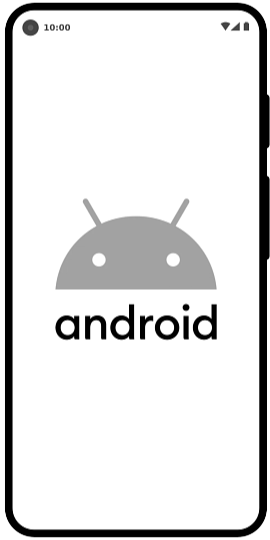
\includegraphics[height=0.5\textheight]{figures/android_device.png}
    \end{figure}
  \end{minipage}

  \note{
    Lets have a quick look at what we will talk about.
    First we will introduce the topic of fingerprintng different devices and mention some methods used in general.
    Then go into detail about sensor fingerprinting, and look at the methodology and the approach we applied.
    We will then present our implementation and show the evaluation steps we took to check if our work is functional.
    In the end we will discuss the limitations of our implementation.
  }
\end{frame}


\section{Introduction}

\begin{frame}{Introduction}
  \begin{minipage}{0.49\textwidth} 
    \begin{itemize}
      \item Misuse of the Android API
      \pause
      \item Used for targeted advertisements
      \pause
      \item Does not require user permission
    \end{itemize}
  \end{minipage}
  \hfill
  \begin{minipage}{0.49\textwidth} 
    \begin{figure}
      \centering
      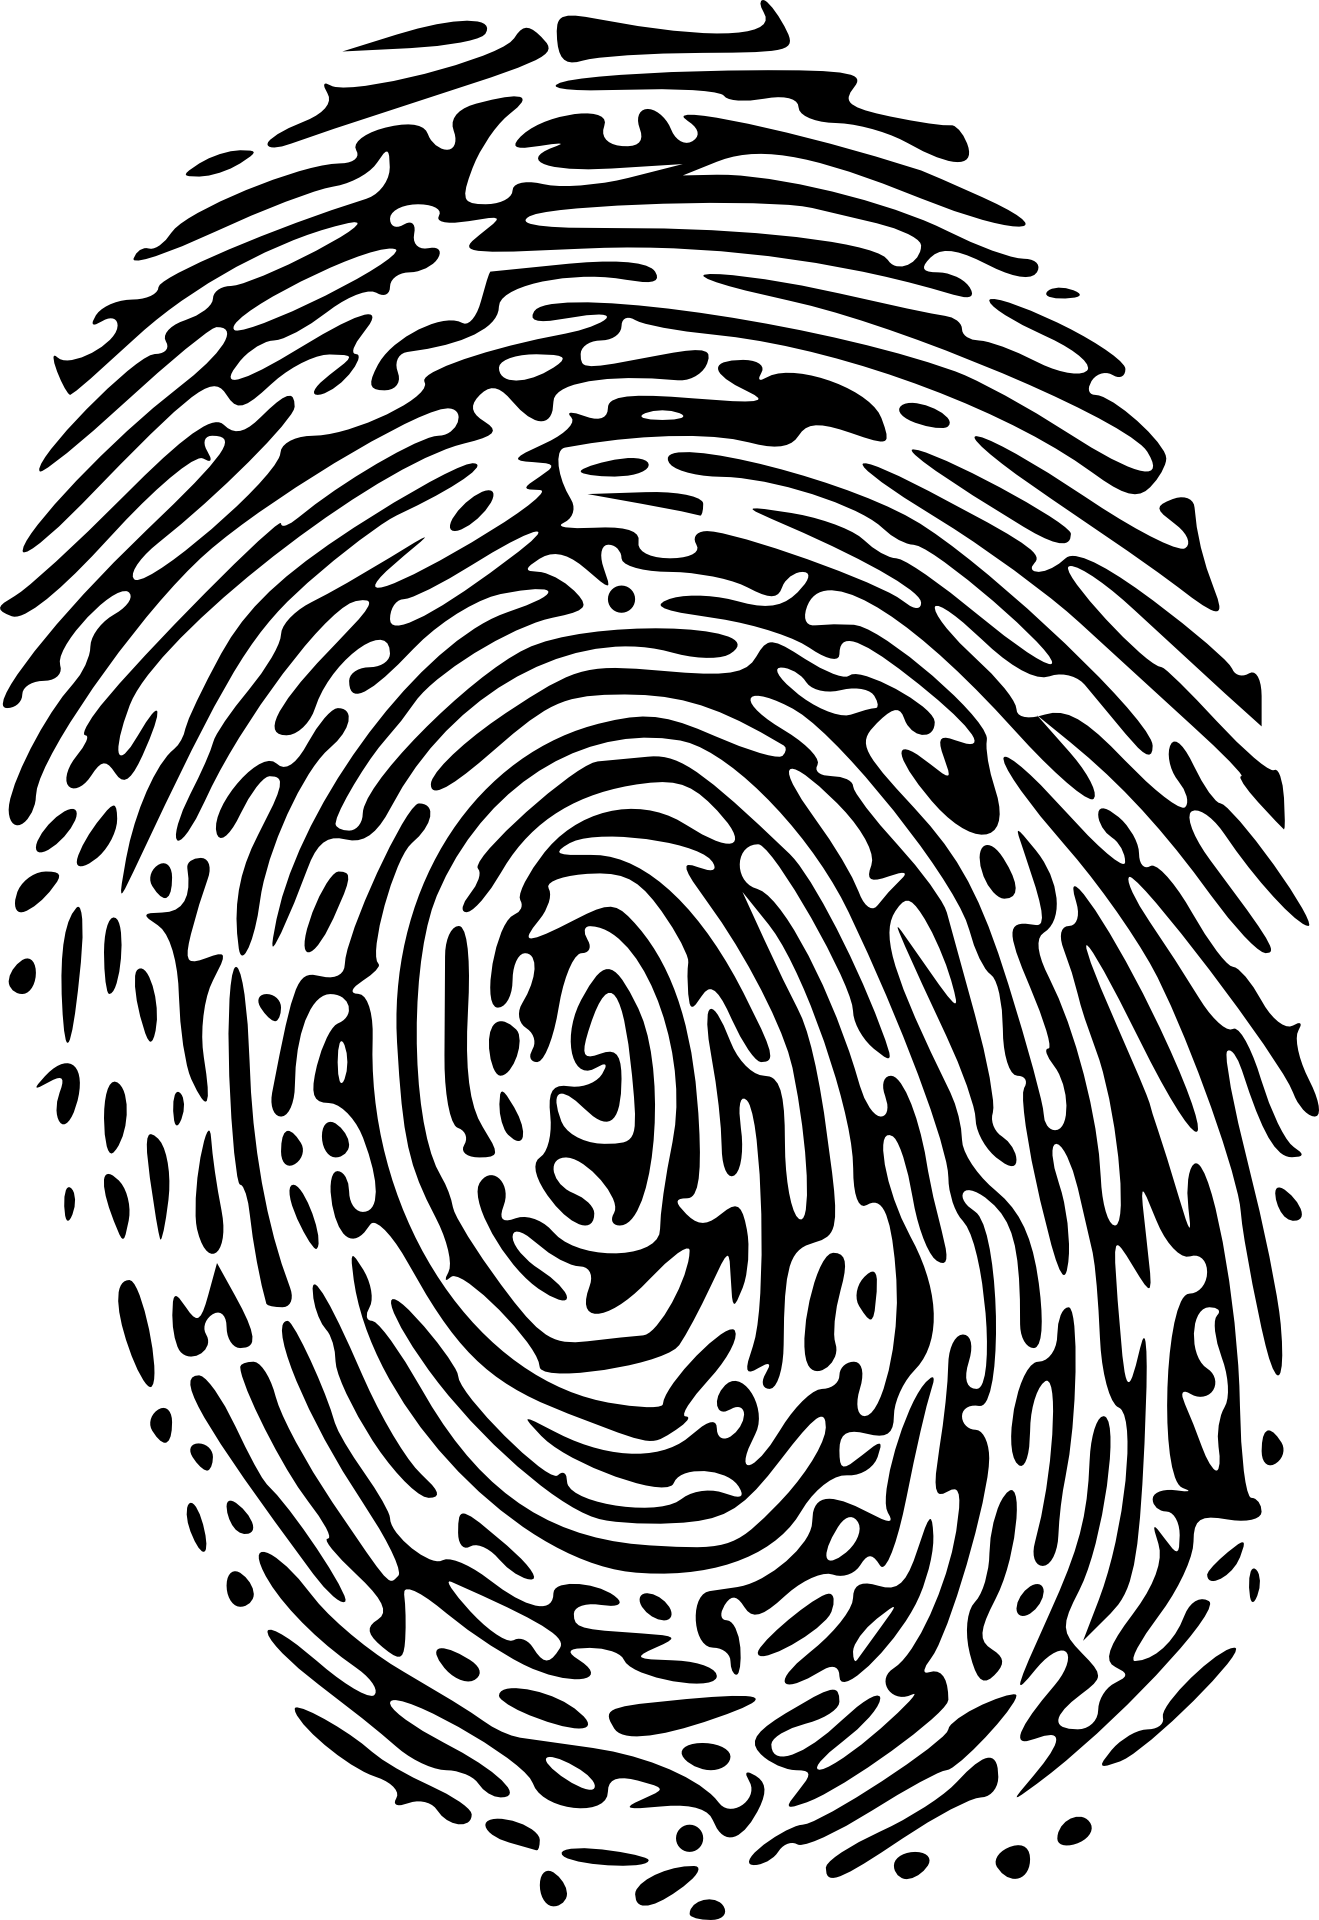
\includegraphics[height=0.5\textheight]{figures/fingerprint.png}
    \end{figure}
  \end{minipage}

  \note<1>{
    Fingerprints are created by misusing the android api in a way it way not intended to.
    The android api is used to query different data from the device.
    Individual data can be requested through the api like it was intended to and used harmlessly.
    But when a multitude of information about the device is requested and is combined it can be harmful.
    The combination of these easily accessed information can be unique to a user and his device.
  }

  \note<2>{
    This unique fingerprint can be used to track users and their habbits.
    This data then can be used for example to create targeted advertisements for individual users.
  }

  \note<3>{
    Many of the required information that are used for the unique fingerprint can be requested through the android api without additional user granted permission.
    Due to the absence of explicit consent and knowledge of the user these permission less fingerprints create a significant privacy threat.
  }
\end{frame}

\section{Background}

\begin{frame}{Smartphone Fingerprinting}
  \begin{minipage}{0.49\textwidth} 
    \begin{itemize}
      \item Similar to browser fingerprinting
      \pause
      \item Not as known as browser fingerprinting
      \pause
      \item Zero permission identifiers
      % \pause
      % \item Personalized configurations
    \end{itemize}
  \end{minipage}
  \hfill
  \begin{minipage}{0.49\textwidth} 
    \begin{figure}
      \centering
      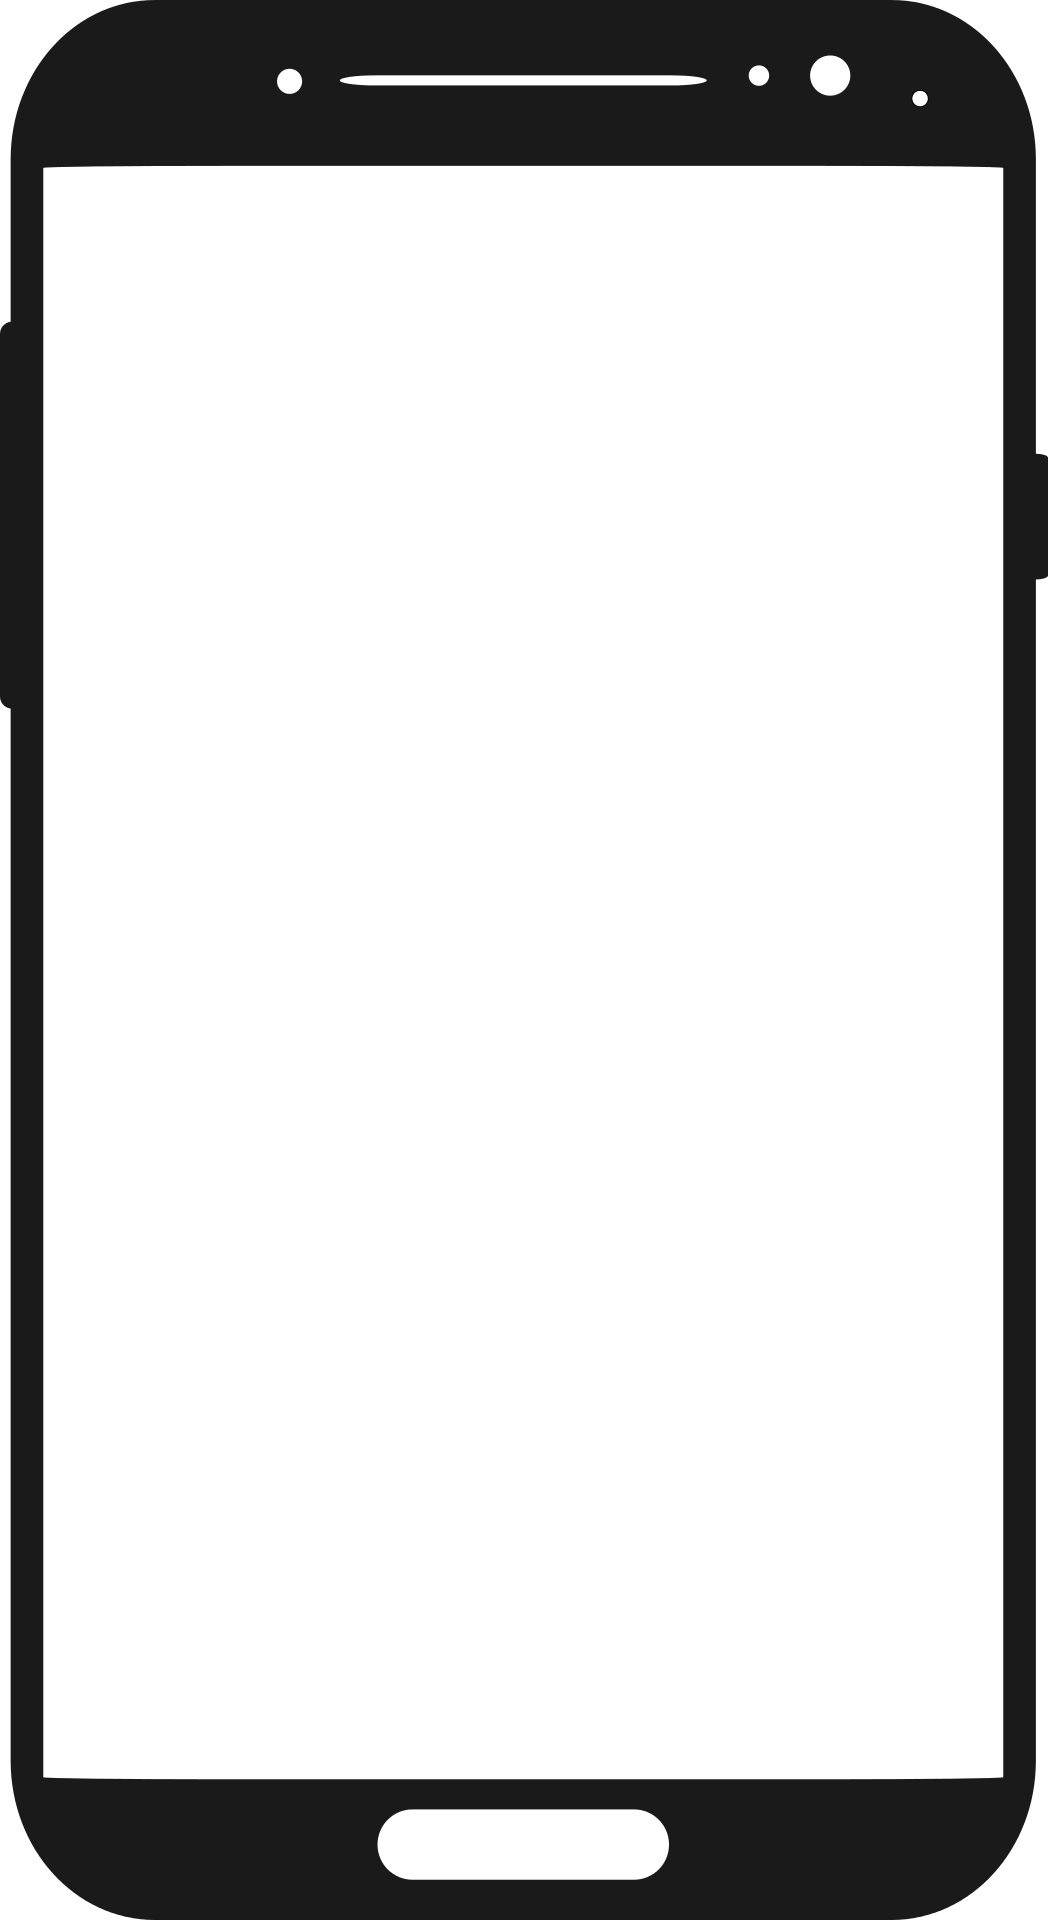
\includegraphics[height=0.5\textheight]{figures/smartphone.png}
    \end{figure}
  \end{minipage}

  \note<1>{
    Smartphone fingerprinting is very similar to browser fingerprinting.
    Browsers can be identified and fingerprinted, by gathering various informations about the screen, installed fonts and extension.
  }

  \note<2>{
    Even though browser fingerprinting is similar to browser fingerprinting and just as a privacy threat it is not as widely known.
    Because it is not as widely known there are currently also a lot less of protections on devices.
  }

  \note<3>{
    To create a fingerprint of a mobile device in many cases zero permission identifiers are used.
    These can be information about the device, configurations and different sensors.
  }
\end{frame}


\section{Sensor Fingerprinting}

\begin{frame}{Fingerprinting Sensors}
  \begin{minipage}{0.49\textwidth} 
    \begin{itemize}
      \item Measurement inaccuracy of sensors
      \pause
      \item Simple to fingerprint via machine learning algorithmus
      \pause
      \item Constant over the sensors lifetime
    \end{itemize}
  \end{minipage}
  \hfill
  \begin{minipage}{0.49\textwidth}
    \begin{figure}
      \centering
      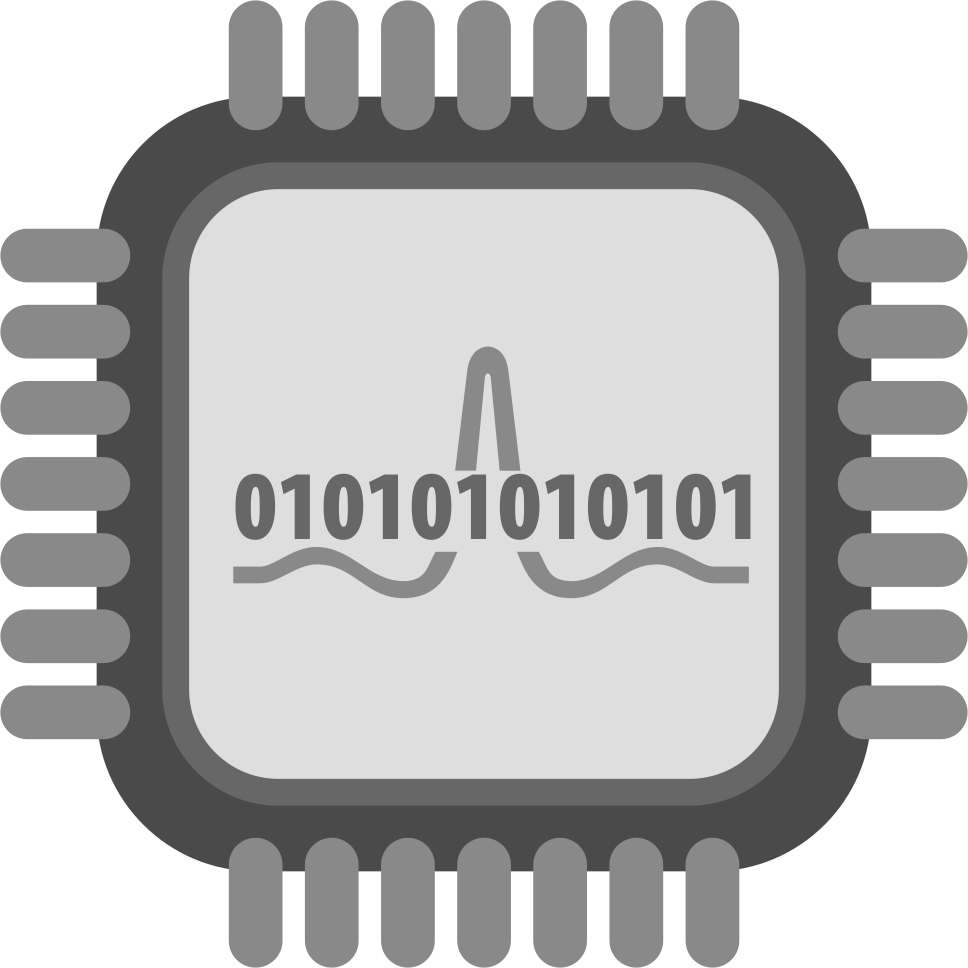
\includegraphics[height=0.5\textheight]{figures/analog.png}
    \end{figure}
  \end{minipage}

  \note<1>{
    The main topic of ours is to focus on sensor fingerprinting.
    These fingerprints are created by reading the sensor values and determining the measurement inaccuracy.
    This measurement error is created due to the not perfect manufacturing processes of the sensors.
    Multiple sensors can be used for fingerprinting, such as gyroscopes and accelerometers.
    These are not the only sensors, that can be used but are already present in nearly all of the mobile devices today and we will focus on these sensors in the following.
  }

  \note<2>{
    Fingerprinting sensors can be done in multiple ways.
    The most simple one is to train a machine learning algorthim to match the recorded sensor values to the device they were recorded from.
  }

  \note<3>{
    It has been already proven by multiple pappers, that these fingerprints based on the builtin sensor error are constant over the lifetime of a sensor.
    These fingerprints are also unique enough to be used to identify the device they were recorded from.
  }
\end{frame}


\section{Methodology}

\begin{frame}{Main Question}
  \begin{minipage}{0.65\textwidth} 
    How to protect against sensor fingerprinting
  \end{minipage}
  \hfill
  \begin{minipage}{0.34\textwidth} 
    \begin{figure}
      \centering
      
\includegraphics[height=0.5\textheight]{figures/question.png}
    \end{figure}
  \end{minipage}

  \note{
    The main question of us is:
    How to protect against sensor fingerprinting?
    There have been already some papers that focused on the problem of sensor fingerprinting.
    Some of these also had some proposed solutions to mitigate the privacy risk.
  }
\end{frame}

\begin{frame}{Proposed Solutions}
  \begin{minipage}{0.49\textwidth} 
    Calibration
    \begin{itemize}
      \item Systematic adjustment of sensor readings
      \item Correcting the sensor data
    \end{itemize}
  \end{minipage}
  \hfill
  \begin{minipage}{0.49\textwidth} 
    Noise Generation
    \begin{itemize}
      \item Introduces variability into the sensor data
      \item Masks the original values
    \end{itemize}
  \end{minipage}

  \note{
    There are mainly two proposed solutions.
    Calibration and noise generation, which each having a different approach.
    The first we will look at is calibration.
    We can mitigate the builtin factory imporfections of a sensor by recalibarting it to correct the error.
    Noise geration on the other hand makes the error larger and random by introducing variability into the sensor data to mask the original value.
  }
\end{frame}

\begin{frame}{Challenges}
  \begin{minipage}{0.49\textwidth} 
    Calibration
    \begin{itemize}
      \item Requires user awareness\\and interaction
      \item Requires precision
    \end{itemize}
  \end{minipage}
  \hfill
  \begin{minipage}{0.49\textwidth} 
    Noise Generation
    \begin{itemize}
      \item Degrade the functionality of applications
      \item Code has to be modified
    \end{itemize}
  \end{minipage}

  \note{
    Both of the proposed solutions have their respective challages.
    Calibration requires user awareness and interaction.
    They have to actively and precisely calibrate their sensors to get rid of and not just change the sensor imperfections.
    Noise generation does not require user interaction, but due to the noise and decreased accuracy of the sensor data applications would also decrease their functionality.
    Also in order to introduce the masking noise into the application the code would need to be modified.
  }
\end{frame}


\section{Approach}

\begin{frame}{Our Methodology}
  \begin{minipage}{0.49\textwidth} 
    \begin{itemize}
      \item Noise Generation
      \item Patch application vie A2P2 framework
    \end{itemize}
  \end{minipage}
  \hfill
  \begin{minipage}{0.49\textwidth} 
    \begin{figure}
      \centering
      
\includegraphics[height=0.5\textheight]{figures/android.png}
    \end{figure}
  \end{minipage}

  \note{
    Our nethodology uses the proposed noise generation, to mask the builtin error of sensors.
    We choose this because we believe it to be much easier to scale up then to rely on the users precicion to calibrate their device to perfection.
    To introduce our custom code responsible for the noise generation we are using the android application pipeline, short a2p2, which enables easy integration into a number of android apps.
  }
\end{frame}

\begin{frame}{Modifying the Sensor API}
  \begin{minipage}{0.49\textwidth} 
    \begin{itemize}
      \item Intercept calls to registerListener method
      \item Provide modified values to onSensorChanged method
    \end{itemize}
  \end{minipage}
  \hfill
  \begin{minipage}{0.49\textwidth} 
    \begin{figure}
      \centering
      
\includegraphics[height=0.5\textheight]{figures/code.png}
    \end{figure}
  \end{minipage}

  \note{
    To replace the original sensor values with our masked ones we have to modify the sensor api.
    We have intercept calls to the registerListener function in order to let our masking class recieve the sensor values instead of the original calling method.
    Also we will need to implement the onSensorChanged method to pass the recieved sensor value from the system after adding noise to the original calling method.
  }
\end{frame}

\begin{frame}{Noise Generation}
  \begin{minipage}{0.49\textwidth} 
    \begin{itemize}
      \item Adds random gain and offset to every value
      \item Masks values
      \item Loss of precision
    \end{itemize}
  \end{minipage}
  \hfill
  \begin{minipage}{0.49\textwidth} 
    \begin{figure}
      \centering
      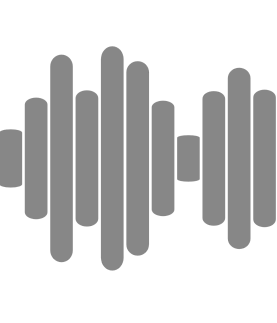
\includegraphics[height=0.5\textheight]{figures/noise.png}
    \end{figure}
  \end{minipage}

  \note{
    In our approach the selected noise generation adds a random gain and offset to every single sensor value, masking the original value with their error.
    Due to applied noise there will be a loss of precision in the sensor values degrading app functionality.
  }
\end{frame}

\section{Implementation}

\begin{frame}<1>[label=impl]{Implementation}
  \begin{minipage}{0.49\textwidth} 
    \begin{itemize}
      \item Intercept Method
      \pause
      \item Noise Generating Function
      \pause
      \item Random Value Generation Function
    \end{itemize}
  \end{minipage}
  \hfill
  \begin{minipage}{0.49\textwidth} 
    \begin{figure}
      \centering
      
\includegraphics[height=0.5\textheight]{figures/java.png}
    \end{figure}
  \end{minipage}

  \note<1>{
    Our implementation has some fundamental methods which ensure the tunctionality of our patch.
    The first is the intercept method.
  }

  \note<2>{
    An other important part of our implementation is the noise generating function.
  }

  \note<3>{
    The most important function is the random value generation function, which ensures the randomnes of the values used for the noise generation to prevent newly created fingerprintable features.
  }
\end{frame}

\begin{frame}{Intercept Method}
  \begin{textblock*}{\textwidth}(30pt,50pt)
  \begin{figure}
    \centering
    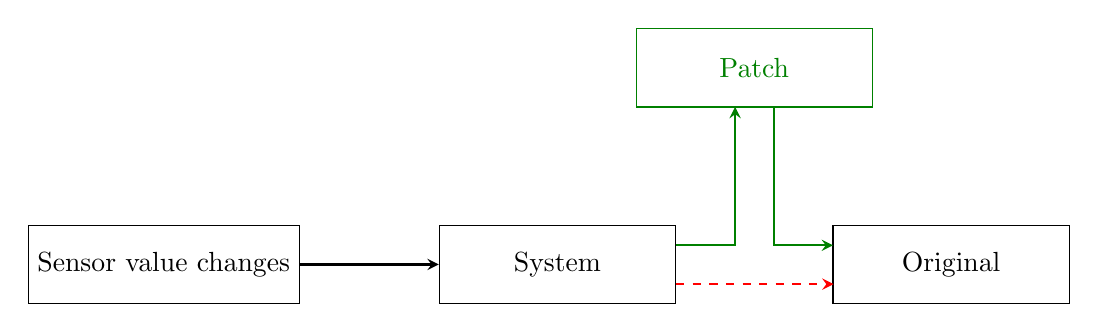
\begin{tikzpicture}
      \tikzstyle{process} = [rectangle, minimum width=3cm, minimum height=1cm, text centered, draw=black]

      \node (sensor) [process] at (0,0) {Sensor value changes};
      \node (system) [process] at (5,0) {System};
      \node (patch) [process, black!50!green] at (7.5,2.5) {Patch};
      \node (function) [process] at (10,0) {Original};

      \draw [thick, ->, >=stealth] (sensor) -- (system);
      \draw [thick, ->, >=stealth, red, dashed] (system.east)+(0,-0.25) -- +(2,-0.25);
      \draw [thick, ->, >=stealth, black!50!green] (system.east)+(0,0.25) -| +(0.75,2);
      \draw [thick, ->, >=stealth, black!50!green] (patch.south)+(0.25,0) |- +(1,-1.75);
    \end{tikzpicture}
    \caption{The function calls from the system are intercepted by our patch and forwarded after modification to the original function.}
  \end{figure}
  \end{textblock*}

  \note{
    The intercept method is responsible for intercepting the sensor values from the system before reaching the original method and forward them to our patch.
    Our patch then generates and applies noise to this recieved values and passes them to the original method.
  }
\end{frame}

\againframe<2>{impl}

\begin{frame}{Noise Generating Function}
  \begin{center}
    \begin{align*}
      value_{new} = \frac{(value_{old} - offset_{sensor})}{gain_{sensor}}
    \end{align*}
  \end{center}

  \note{
    By subtracting a random offset and divinding a random gain from the original value we genarate the new obfuscated sensor value.
    The random values of the offset and gain are generated from a carefully selected range responsible for the amplitude of the nosie.
  }
\end{frame}

\againframe<3->{impl}

\begin{frame}{Application of Patch}
  \begin{minipage}{0.49\textwidth} 
    \begin{itemize}
      \item Straightforward application 
      \item Only requirements are
      \begin{itemize}
        \item JAVA JRE
        \item A2P2
        \item APK to be modified
      \end{itemize}
    \end{itemize}
  \end{minipage}
  \hfill
  \begin{minipage}{0.49\textwidth} 
    \begin{figure}
      \centering
      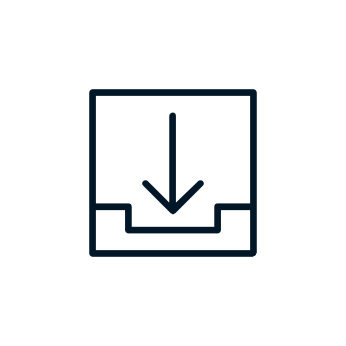
\includegraphics[height=0.5\textheight]{figures/download.png}
    \end{figure}
  \end{minipage}

  \note{
    The application of our patch is very straightforward.
    We only need to install JAVA runtime environment and download the latest a2p2 release and the apk of the app the we want to patch.
    If all these reqirements are met the app can be patched by executing a simple single command.
  }
\end{frame}


\section{Evaluation}

\begin{frame}<1>[label=testing]{Testing}
  \begin{minipage}{0.49\textwidth} 
    \begin{itemize}
      \item<1-> Functionality
      \item<2-> Effectiveness
      \item<3-> Usabilty
    \end{itemize}
  \end{minipage}
  \hfill
  \begin{minipage}{0.49\textwidth} 
    \begin{figure}
      \centering
      
\includegraphics[height=0.5\textheight]{figures/test-tube.png}
    \end{figure}
  \end{minipage}

  \note<1>{
    To determine if our patch mitigates fingerprintability we have to perform some tests.
    To check the functionality of our patch and controll that sensor values are intercepted and modified before passing them to the original function.  
  }

  \note<2>{
    Then we have to check the effectiveness of our patch in mitigating fingerprintability.
  }

  \note<3>{
    We also tested if the patched apps retained their functionality and usabilty.
    To test this we patched a motion controlled game and were still able to play the game without significant problems.
  }
\end{frame}

\begin{frame}{Functionality}
  \begin{minipage}{0.49\textwidth}
    \begin{figure}
      \centering
      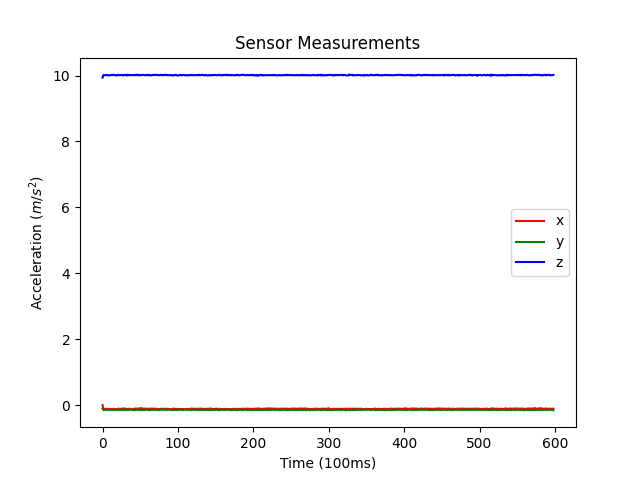
\includegraphics[height=0.45\textheight]{figures/SensorValuesBefore.png}
      \caption{recorded values before the patch}
    \end{figure}
  \end{minipage}
  \hfill
  \begin{minipage}{0.49\textwidth}
    \begin{figure}
      \centering
      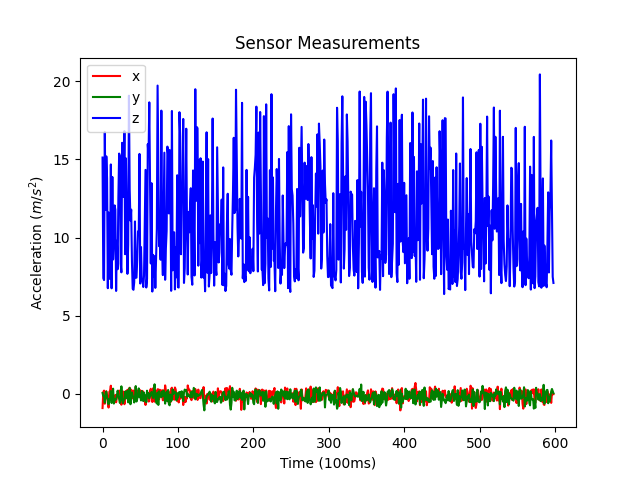
\includegraphics[height=0.45\textheight]{figures/SensorValuesAfter.png}
      \caption{recorded values after the patch}
    \end{figure}
  \end{minipage}

  \note{
    We do this by recording sensor values over a small period of time with an android app.
    Then we apply our patch to the app we used to record the values and compare the recorded results.
    As we can see the recorded sensor values were constant before the patch but got inconsistant after the application of our patch.
  }
\end{frame}

\againframe<2>{testing}

\begin{frame}{Effectiveness}
  \begin{minipage}{0.49\textwidth}
    \begin{figure}
      \centering
      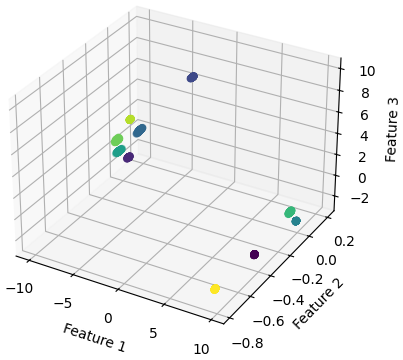
\includegraphics[height=0.45\textheight]{figures/knn_before.png}
      \caption{knn decision boundaries before the patch}
    \end{figure}
  \end{minipage}
  \hfill
  \begin{minipage}{0.49\textwidth}
    \begin{figure}
      \centering
      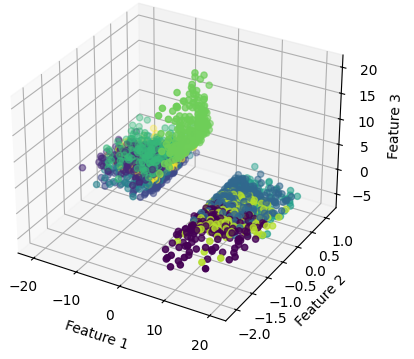
\includegraphics[height=0.45\textheight]{figures/knn_after.png}
      \caption{knn decision boundaries after the patch}
    \end{figure}
  \end{minipage}

  \note{
    To test this we trained a knn machine leaarning model with the recorded sensor values before and after the application of our patch.
    We can observe that before our patch the decision boundaries of the trained model were very prominant and easily differentiable.
    This lead to 100\% accuracy in the predictions of the model.
    After our patch the decision boundaries were not that easily distinguisable and the trained models accuracy decreased noticably.
  }
\end{frame}

\againframe<3->{testing}

\begin{frame}{Noise Level Adjustment}
  \begin{minipage}{0.49\textwidth} 
    \begin{itemize}
      \item Increasing noise decreases fingerprintability
      \item Increasing noise decreases functionality
    \end{itemize}
  \end{minipage}
  \hfill
  \begin{minipage}{0.49\textwidth} 
    \begin{figure}
      \centering
      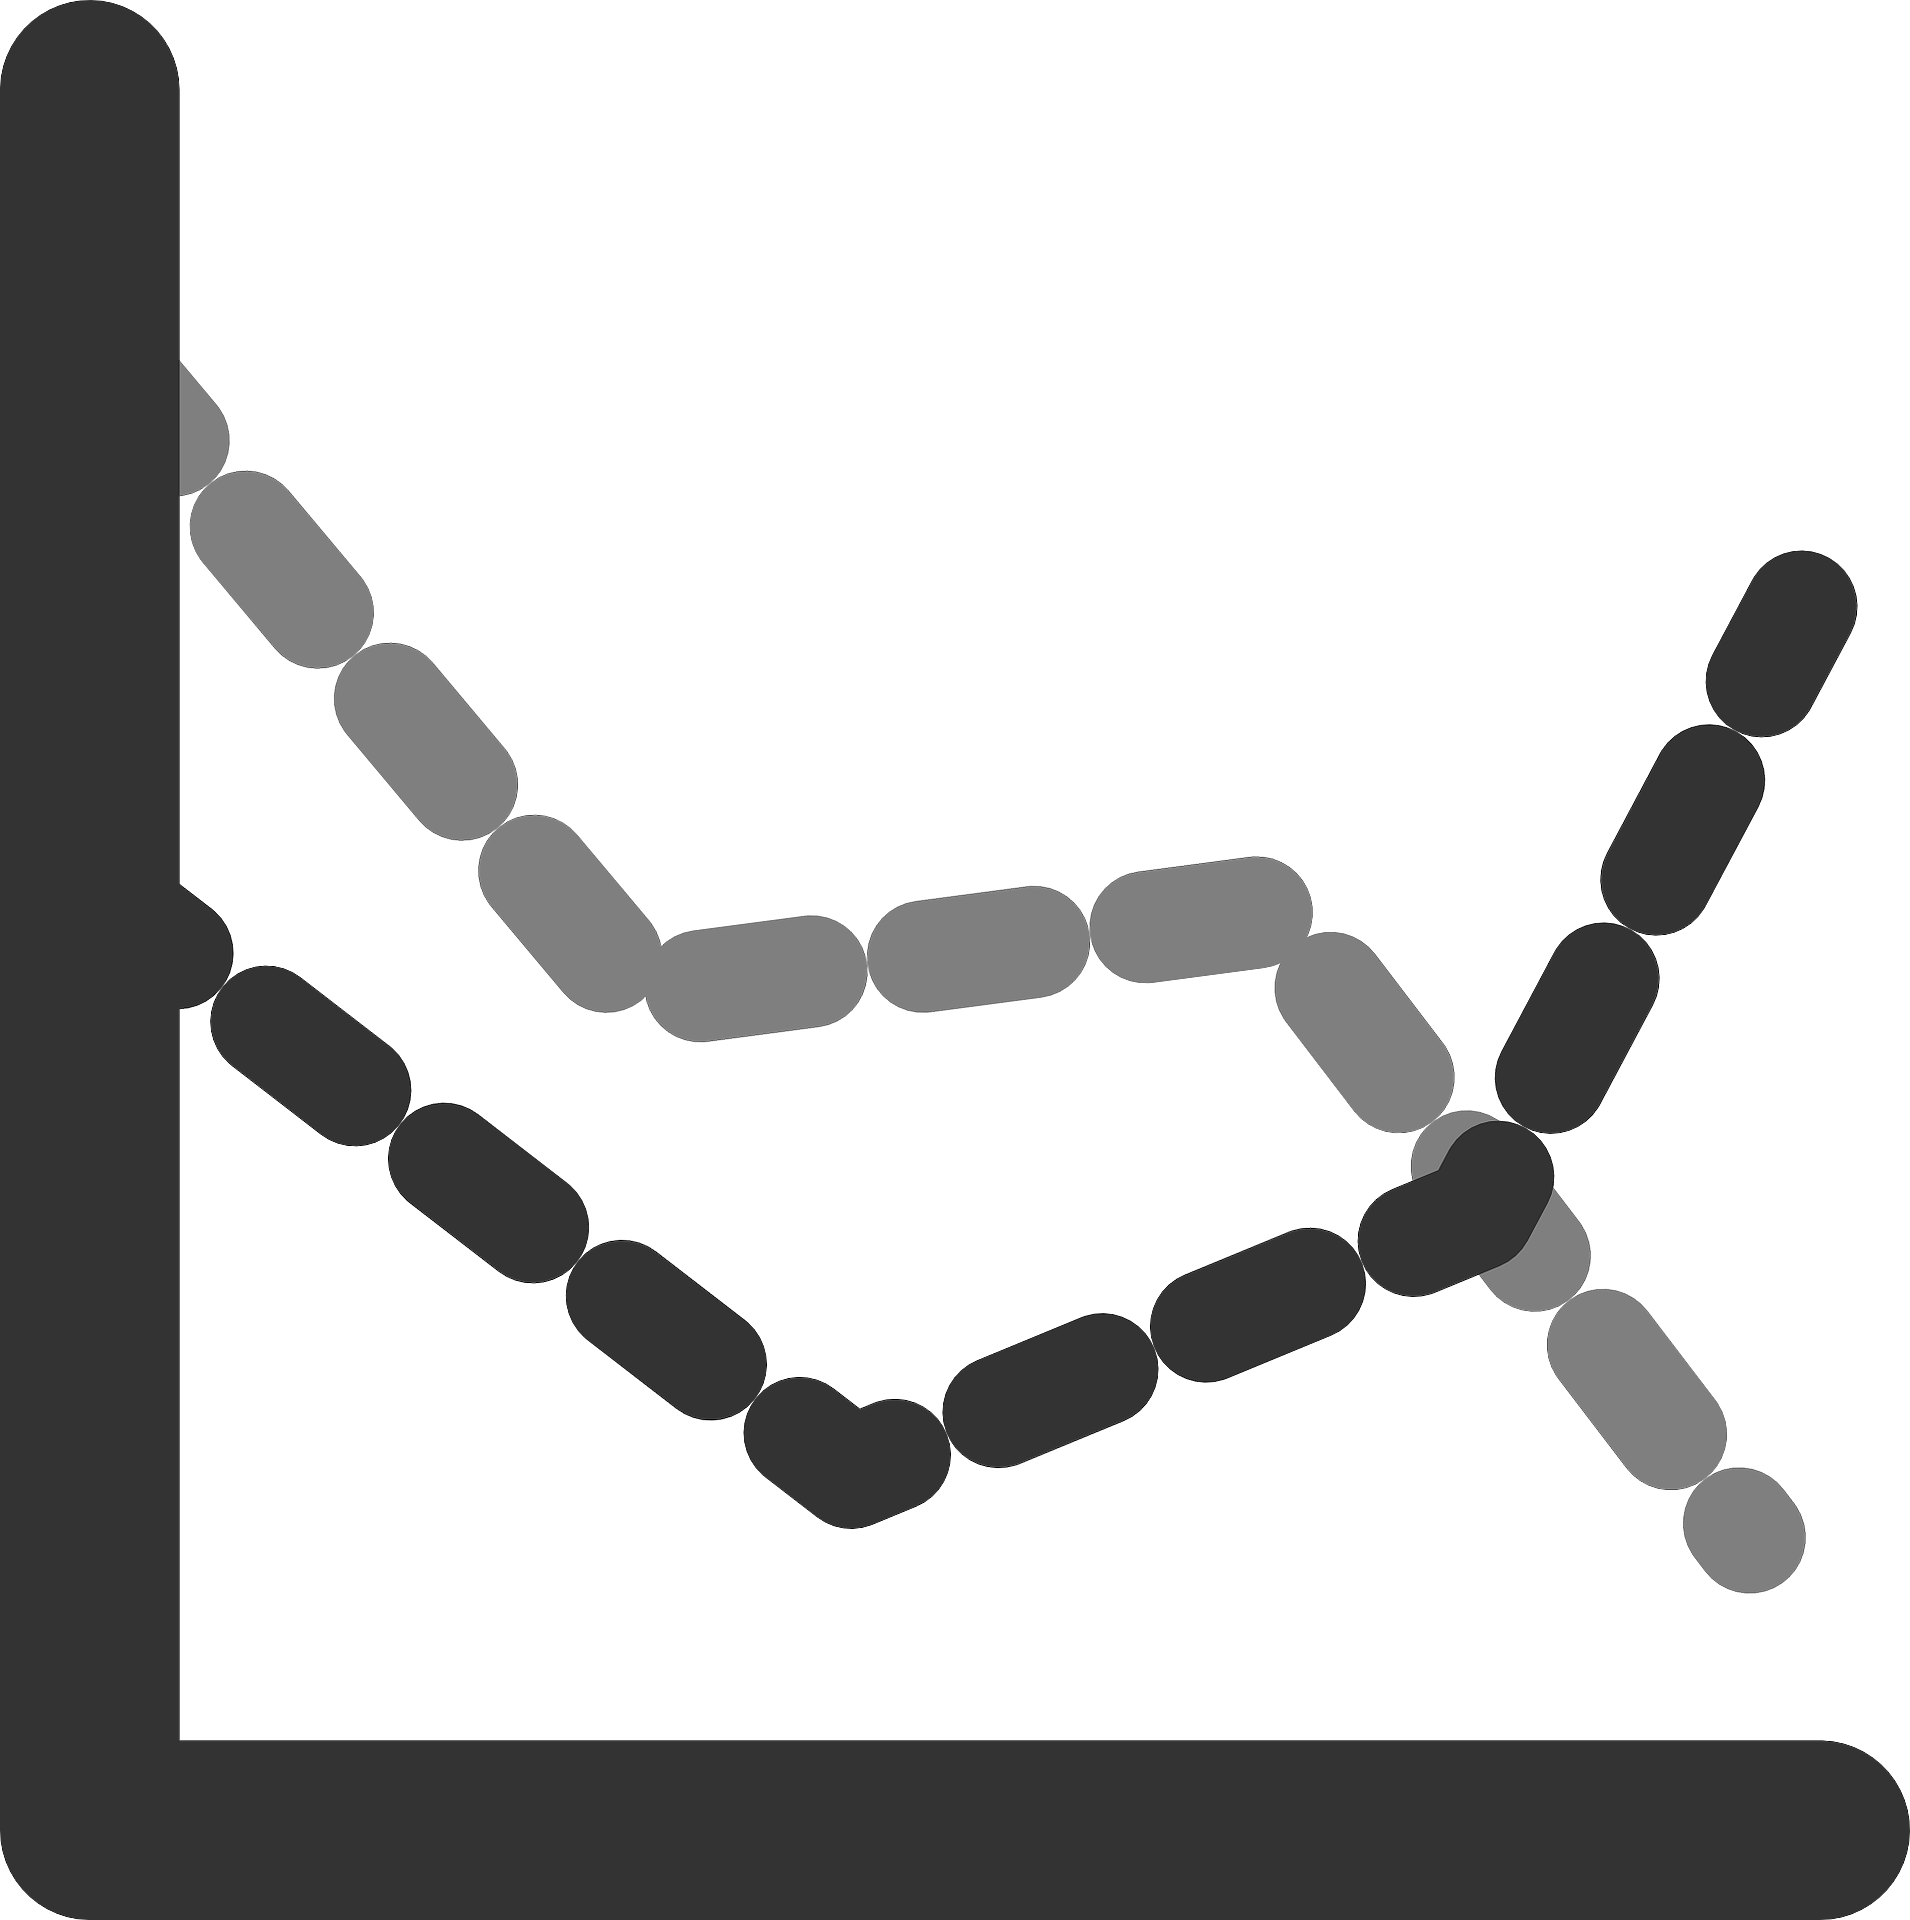
\includegraphics[height=0.5\textheight]{figures/graph.png}
    \end{figure}
  \end{minipage}

  \note{
    We also evaluated the level of the applied noise.
    Increasing the nosie we noticed it decreased the fingerprintability, but also decreased the apps functionality significantly.
    We have to balance the level of the applied nosie in order to have the most effective mitigation of fingerprinting but stil retaining the apps functionality.
  }
\end{frame}

\section{Discussion \& Limitations}

\begin{frame}{Discussion \& Limitations}
  \begin{minipage}{0.49\textwidth} 
    \begin{itemize}
      \item Limited amount of test devices
      \item Could not be done sufficiently due to limited access to supported hardware
    \end{itemize}
  \end{minipage}
  \hfill
  \begin{minipage}{0.49\textwidth} 
    \begin{figure}
      \centering
      
\includegraphics[height=0.5\textheight]{figures/comments.png}
    \end{figure}
  \end{minipage}

  \note{
    Our test was done with a limited number of devices in a controlled environment.
    But we are confident that based on our findings and other pubished papers our patch would also mitigate sensor fingerprintability on a larger scale in an everyday environment.
  }
\end{frame}

\section*{}

\begin{frame}{Conclusion}
  \begin{minipage}{0.49\textwidth} 
    \begin{itemize}
      \item Easy application of the patch 
      \item Masking the sensor values decreases fingerprintability
    \end{itemize}
  \end{minipage}
  \hfill
  \begin{minipage}{0.49\textwidth} 
    \begin{figure}
      \centering
      
\includegraphics[height=0.5\textheight]{figures/androguard.png}
    \end{figure}
  \end{minipage}

  \note{
    We believe that our implementation of androguard is a possible solution to lower privacy violations.
    By easily applying our patch to applications and masking the builtin error of sensors with added nosie we mitigate sensor fingerprinting on android.
  }
\end{frame}

% \begin{frame}{Bibliography}
%   ...
% \end{frame}

\end{document}
